\documentclass[a4paper,12pt]{article}
\usepackage{a4wide}
\usepackage[pdftex]{hyperref}
\usepackage[german]{babel}
\usepackage[utf8]{inputenc}
\usepackage{amssymb}
\usepackage{csquotes}
\usepackage{wrapfig}
\usepackage{graphicx}
\usepackage{multicol}
\usepackage{amsmath}
\usepackage{enumitem}
\usepackage{polynom}
\usepackage{siunitx}

\setlength{\marginparsep}{1 cm}
\setlength{\topmargin}{-0.6in}
\setlength{\textheight}{9.5in}
\pagestyle{plain}

\polyset{%
   style=C,
   delims={\big(}{\big)},
   div=:
}

% Polynomial long division
\polyset{%
	style=C,
	delims={\big(}{\big)},
	div=:
}

% Differential operator
\newcommand{\diff}[1]{\:\mathrm{d}{#1}}
\newcommand{\pdd}[2]{\frac{\partial #1}{\partial #2}}
\newcommand{\pddn}[3]{\frac{\partial^{#1} #2}{\partial #3^{#1}}}
\newcommand{\dd}[2]{\frac{\mathrm{d}{#1}}{\mathrm{d}{#2}}}
\newcommand{\ddn}[3]{\frac{\mathrm{d}^{#1}{#2}}{\mathrm{d}{#3^{#1}}}}

% N-th root
% \nroot{3}{27}
\newcommand*{\nroot}[2]{\sqrt[\leftroot{-1}\uproot{2}#1]{#2}}
\newcommand*{\ncroot}[4]{\sqrt[\leftroot{#1}\uproot{#2}#3]{#4}}

% 2 component vector
% \tvect{1}{-1}
% \tvec{1}{-1}
\newcommand{\tvect}[2]{%
   \ensuremath{\Bigl(\negthinspace\begin{smallmatrix}#1\\#2\end{smallmatrix}\Bigr)}}
\newcommand{\tvec}[2]{%
    \ensuremath{\left(\negthinspace\begin{matrix}#1\\#2\end{matrix}\right)}}

% 3 component vector
% \rvect{1}{-1}{0}
% \rvec{1}{-1}{0}
\newcommand{\rvect}[3]{%
   \ensuremath{\Bigl(\negthinspace\begin{smallmatrix}#1\\#2\\#3\end{smallmatrix}\Bigr)}}
\newcommand{\rvec}[3]{%
    \ensuremath{\left(\negthinspace\begin{matrix}#1\\#2\\#3\end{matrix}\right)}}

% Long vector arrow
% \xshlongvec{ABC}

% German-style quotation marks %
\MakeOuterQuote{"}

% Number sets
\newcommand{\N}{\mathbb{N}}
\newcommand{\Z}{\mathbb{Z}}
\newcommand{\Q}{\mathbb{Q}}
\newcommand{\R}{\mathbb{R}}
\newcommand{\C}{\mathbb{C}}

\newcommand{\setzero}{\varnothing}

% Mention (small caps)
\newcommand{\mention}[1]{\textsc{#1}}

% Functions
\newcommand{\asin}[0]{\text{asin}}
\newcommand{\acos}[0]{\text{acos}}
\newcommand{\atan}[0]{\text{atan}}
\newcommand{\sgn}[0]{\text{sgn}}
\newcommand{\grad}[0]{\text{grad}}

% Scale
% Usage in math mode: \Scale[1.5]{...equation...} %
\newcommand*{\Scale}[2][4]{\scalebox{#1}{$#2$}}%

% Units
\newcommand{\um}{\text{m}}
\newcommand{\us}{\text{s}}
\newcommand{\ukm}{\text{km}}
\newcommand{\ukg}{\text{kg}}
\newcommand{\uh}{\text{h}}
\newcommand{\ukmh}{\frac{\ukm}{\uh}}
\newcommand{\umpers}{\frac{\um}{\us}}
\newcommand{\umss}{\frac{\ukm}{\us^2}}
\newcommand{\ukgss}{\frac{\ukg}{\us^2}}
\newcommand{\degrees}[1]{\SI{#1}{\degree}}

% Floor / ceil
\newcommand{\floor}[1]{\left\lfloor #1 \right\rfloor}
\newcommand{\ceil}[1]{\left\lceil #1 \right\rceil}

% Circle characters
\newcommand*\circled[1]{
    \tikz[baseline=(char.base)]{
        \node[shape=circle,draw,inner sep=2pt] (char) {#1};
    }
}



\begin{document}

\begin{center}
  {\bf {\large Aufgabenblatt 3 (MI/IT 2020)}}
\end{center}

% Tasks

\begin{enumerate}

\item Geben Sie irgendeine periodische Funktion an, deren Bildbereich gleich $[8,12]$ ist.


\item 
Gegeben ist die Funktion $f(x,y) = e^{x^2 / y}$.
Betrachten Sie deren Höhenlinie, die durch die Stelle $(x_0|y_0)=(1|2)$ läuft. Skizzieren Sie diese auf dem Bereich $[-2;2]\times[-2;2]$.
Wie sieht die Funktion zu den beiden Seiten der Höhenline hin aus, d.h. in welche Richtung zeigt der Gradient?



\item Der Definitionsbereich und der Wertebereich einer einstelligen Funktion sind jeweils Mengen, die aus reellen Zahlen bestehen. Aus welchen mathematischen Objekte besteht der Definitionsbereich und Wertebereich einer dreistelligen Funktion? Geben Sie den Definitionsbereich für $f(x,y,z) = \frac{y^z}{\ln(|x-2|)\sqrt{x+4})}$ an!

% tangente, diff quot
% tangente, tangentialebene
% beschleunigung aus x(t)
% part. ableitung berechnen
% nabla, gradient, schwarz
% asymmetrie int f(x)-f(-x) dx
% gerichteter flächeninhalt
% gebietsintegral kart. polar
% log. diff (kettenregel) x^x
% ableitung tanh,atanh
% integral sin(x)^2, cos(x)^2, gamma-fkt
% lineare substitution
% extremwert 1d,2d

\end{enumerate}

\newpage

% Solutions

\begin{center}
{\bf {\large Lösungen}}
\end{center}

\begin{enumerate}
	
\item  Der Bildbereich ist nach unten und nach oben beschränkt, es bietet sich also eine modifizierte trigonometrische Funktion an:

Zum Beispiel: $f(x) = 2\sin(x) +10$ oder $g(x) = 2\cos(x) +10$



\item 

Die Höhenlinie ist die Menge aller Punkte $(x,y)$, wo die Funktion den gleichen Funktionswert besitzt, $f(x,y) = const.$ Zur Bestimmung dieser Konstanten setzen wir den Punkt $(x_0,y_0)$ ein:

$f(x,y) = f(1,2)$

$\implies e^{\frac{x^2}{y}} = e^{\frac{1}{2}}$

$\implies \frac{x^2}{y} = \frac{1}{2}$

$\implies y = 2x^2$

Die gesuchte Höhenlinie ist also eine Parabel, die um den Faktor $2$ entlang der y-Achse gestreckt ist.

Zur Bestimmung des Gradienten benötigen wir die partiellen Ableitung nach x und y:

$\frac{\partial f}{\partial x} =  \frac{2x}{y} \cdot e^{\frac{x^2}{y}}$

$\frac{\partial f}{\partial y} =  e^{\frac{x^2}{y}} \cdot (-y^{-2} \cdot x^2) = - \frac{x^2}{y^2} \cdot e^{\frac{x^2}{y}} $

Einsetzen der Höhenlinie $y=2x^2$:

$\frac{\partial f}{\partial x}|_{y=2x^2}=  e^{\frac{x^2}{2x^2}} \cdot \frac{2x}{2x^2} = e^{\frac{1}{2}}\cdot \frac{1}{x}$

$\frac{\partial f}{\partial y}|_{y=2x^2} =  -e^{\frac{x^2}{2x^2}} \cdot \frac{x^2}{4x^4} = -e^{\frac{1}{2}}\cdot \frac{1}{4x^2}$

Der Gradient auf der Höhenlinie zeigt immer in negative y-Achenrichtung (nach unten).

In der rechten Halbebene zeigt er in positive x-Richtung (nach rechts), in der linken Halbebene in negative x-Richtung (nach links).

\begin{figure}[ht]
\centering
  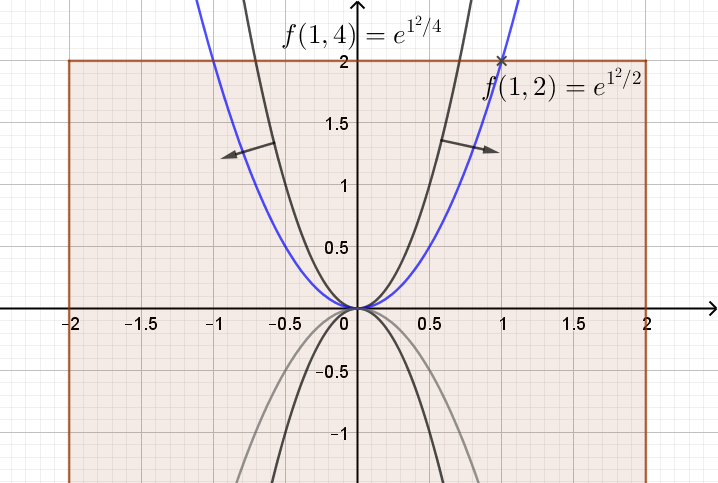
\includegraphics[width=0.4\textwidth]{../pool/ex-graph-contour-1-img-a.png}
  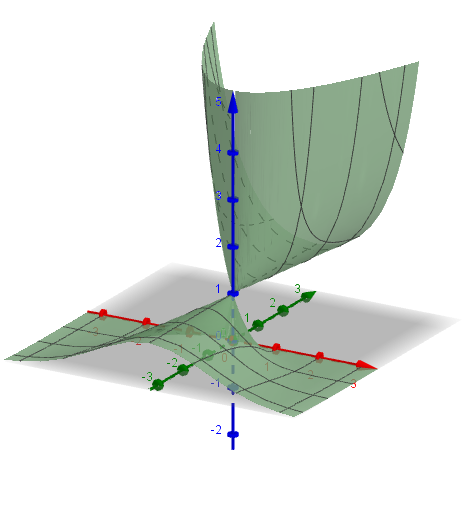
\includegraphics[width=0.4\textwidth]{../pool/ex-graph-contour-1-img-b.png}
  \caption{Höhenlinie mit Gradient zur Höhenlinie $f(x,y)=f(1,2)$ (links) und 3D-Plot davon (rechts)}
\end{figure}



\item Der Definitionsbereich einer dreistelligen Funktion besteht aus 3-Tupeln von reellen Zahlen, welche ein kartesisches Produkt darstellen: $\R\times\R\times\R=\R^3$. Der Wertebereich besteht wie bei einstelligen Funktionen aus reellen Zahlen.

Wir betrachten die Funktion

$$
	f(x,y,z) = \frac{y^z}{\ln(|x-2|)\sqrt{x+4})}
$$

Folgende Einschränkungen gelten:

\begin{itemize}
	\item Das Argument des Logarithmus muss positiv sein, also $x\ne 2$
	\item Das Argument der Wurzel darf nicht negativ sein, also $x \ge -4$
	\item Der Nenner darf nicht identisch $0$ sein. Damit darf das Argument des Logarithmus nicht 1 sein (da $\ln(1) = 0$), also $x \ne 3$ und $x \ne 1$. Andererseits darf auch das Argument der Wurzel nicht $0$ sein, also $x > -4$.
	\item Der Ausdruck $0^0$ ist nicht definiert, daher dürfen $y$ und $z$ nicht beide gleichzeitig identisch $0$ sein.
\end{itemize}

Zusammengefasst erhalten wir also folgenden Definitionsbereich:

$$
	\mathbb{D} = \lbrace (x,y,z) \in \R^3 \hskip 2mm | \hskip 2mm  [x \in (-4,\infty) \setminus \lbrace 1,2,3 \rbrace ] \land [ y \ne 0 \lor z \ne 0 ] \rbrace
$$

\end{enumerate}

\end{document}

